\documentclass[11pt]{article}

\usepackage[letterpaper,margin=0.9in,headheight=15pt]{geometry}
\usepackage[T1]{fontenc}
\usepackage[utf8]{inputenc}
\usepackage{lmodern}
\usepackage{microtype}
\usepackage{amsmath,amssymb,amsthm,mathtools}
\usepackage{booktabs,longtable,tabularx,array,multirow}
\usepackage{graphicx}
\usepackage{xcolor}
\usepackage{caption,subcaption}
\usepackage{float,placeins}
\usepackage{enumitem}
\usepackage{fancyhdr}
\usepackage{hyperref}
\usepackage[nameinlink,noabbrev]{cleveref}
\usepackage{listings}
\usepackage{upquote}
\usepackage{needspace}

\definecolor{Ink}{HTML}{17202A}
\definecolor{Muted}{HTML}{566573}
\definecolor{Blue}{HTML}{2E86AB}
\definecolor{Teal}{HTML}{2A9D8F}
\definecolor{Orange}{HTML}{F4A261}
\definecolor{Red}{HTML}{E76F51}
\definecolor{Purple}{HTML}{7D3C98}
\definecolor{Paper}{HTML}{FAFAF7}
\definecolor{SoftBlue}{HTML}{EAF3F7}
\definecolor{SoftTeal}{HTML}{EAF5F2}
\definecolor{SoftOrange}{HTML}{FCF1E8}
\definecolor{SoftRed}{HTML}{FBEDEA}

\hypersetup{
  colorlinks=true,
  linkcolor=Blue,
  citecolor=Purple,
  urlcolor=Blue,
  pdftitle={The ABC Three-Channel Signal: A Companion Verification},
  pdfauthor={Komorebi P.}
}

\pagestyle{fancy}
\fancyhf{}
\fancyhead[L]{\small The ABC Three-Channel Signal}
\fancyhead[R]{\small Companion Verification}
\fancyfoot[C]{\thepage}

\setlength{\parindent}{0pt}
\setlength{\parskip}{0.62em}
\setlist[itemize]{leftmargin=1.45em,itemsep=0.25em,topsep=0.25em}
\setlist[enumerate]{leftmargin=1.65em,itemsep=0.25em,topsep=0.25em}

\newtheorem{theorem}{Theorem}[section]
\newtheorem{proposition}[theorem]{Proposition}
\newtheorem{lemma}[theorem]{Lemma}
\newtheorem{corollary}[theorem]{Corollary}
\newtheorem{definition}[theorem]{Definition}
\newtheorem{remark}[theorem]{Remark}
\newtheorem{claim}[theorem]{Claim}

\newcommand{\rad}{\operatorname{rad}}
\newcommand{\SNF}{\operatorname{SNF}}
\newcommand{\DFT}{\operatorname{DFT}}
\newcommand{\Tr}{\operatorname{Tr}}
\newcommand{\ord}{\operatorname{ord}}
\newcommand{\Norm}{\operatorname{N}}
\newcommand{\Z}{\mathbb Z}
\newcommand{\Q}{\mathbb Q}
\newcommand{\C}{\mathbb C}
\newcommand{\F}{\mathcal F}
\newcommand{\calC}{\mathcal C}
\newcommand{\calM}{\mathcal M}
\newcommand{\bbone}{\mathbf 1}

\newenvironment{statusbox}[2]{%
  \par\medskip\noindent
  \begin{minipage}{\textwidth}
  \def\statuscolor{#1}%
  \color{\statuscolor}\hrule height 1.2pt\relax
  \vspace{0.45em}
  {\bfseries #2}\par\smallskip
  \color{Ink}%
}{%
  \par\vspace{0.35em}
  \color{\statuscolor}\hrule height 1.2pt\relax
  \end{minipage}
  \par\medskip
}

\lstdefinestyle{companion}{
  language=Python,
  basicstyle=\ttfamily\scriptsize,
  keywordstyle=\color{Purple}\bfseries,
  commentstyle=\color{Muted}\itshape,
  stringstyle=\color{Teal},
  numbers=left,
  numberstyle=\tiny\color{Muted},
  stepnumber=1,
  numbersep=8pt,
  frame=single,
  rulecolor=\color{Muted!40},
  breaklines=true,
  breakatwhitespace=false,
  showstringspaces=false,
  tabsize=4,
  columns=fullflexible,
  keepspaces=true,
  backgroundcolor=\color{Paper}
}

\title{\vspace{-1.5cm}\textbf{The ABC Three-Channel Signal}\\[0.3em]
\Large A Companion Verification of the COS, Eisenstein, Smith, and $3$-Isogeny Construction}
\author{Komorebi P.}
\date{July 2026}

\begin{document}
\maketitle

\begin{abstract}
This companion checks the chain of claims that begins with the observation that the recent arithmetic construction resembles the Fourier cosine method and ends with a three-channel perfect-reconstruction block attached to a primitive relation $a+b=c$.  The purpose is not to make the construction sound stronger than it is.  The purpose is to separate four things that had begun to run together: ideas supported by the four supplied COS and spectral sources, identities proved directly in this companion, statements checked by exact computation, and proposals that remain open.

The main algebraic claims survive the audit.  The signal
\[
  \mathbf s(a,b,c)=(ac,bc,-ab)^T
\]
has zero nontrivial cyclic autocorrelation exactly when $a+b=c$.  Equivalently, its three-point periodogram is flat.  The associated circulant matrix satisfies an exact perfect-reconstruction identity and, for a primitive triple, has Smith normal form
\[
  \operatorname{diag}(1,A,A^2),\qquad A=a^2+ab+b^2.
\]
The two nonconstant Fourier modes are $z^2$ and $\bar z^2$ for the Eisenstein packet $z=a+b\zeta$.  Its third harmonic produces the classical Frey invariants.  The three sector points on the Mordell curve $V^2=U^3+(4abc)^2$ form one rational $3$-torsion orbit and map under the standard $3$-isogeny to the single invariant point $(4A,-4L)$.

The audit also makes two corrections explicit.  A factor such as $1/(q-1)$ in a proposed transformed Ramanujan filter is not an intrinsic invariant until a concrete averaging measure is defined.  The proposed double-atlas expansion theorem is still a research target.  None of the verified identities is a proof of the $abc$ conjecture.
\end{abstract}

\begin{statusbox}{Teal}{Verdict}
The central finite-dimensional identities are correct.  They were proved symbolically, checked on $250$ randomly generated primitive triples, checked on six worked examples, and compared with direct Smith-normal-form calculations.  The Eisenstein representation formula was also checked by brute force for every $1\leq A\leq400$.  The source papers support the transform and recursion principles, but they do not contain the arithmetic theorems proved here.
\end{statusbox}

\begin{statusbox}{Red}{Claim boundary}
This document does not claim a proof of $abc$.  It does not claim a uniform double-atlas expansion theorem.  It does not treat a proposed Ramanujan attenuation factor as canonical before the underlying transfer measure has been defined.  Those points are kept visible rather than hidden in the notation.
\end{statusbox}

\tableofcontents
\clearpage

\section{Why this companion was needed}

The last stage of the project moved quickly.  A numerical analogy with the COS method became a finite Fourier identity, then a circulant perfect-reconstruction block, then an Eisenstein norm, and finally a rational $3$-isogeny connecting a Mordell curve to the Frey invariants.  Each step was plausible.  Plausibility is not the same as verification.

I therefore went back through the construction from the beginning.  Every displayed identity in the main theorem chain was either expanded symbolically or reduced to a short exact proof.  The computational tests were then used as a guard against sign errors, ordering errors in the discrete Fourier transform, and incorrect normalizations in the isogeny formulas.  This matters here because one wrong sign in the third harmonic changes $c_6$, while one wrong ordering of the DFT changes which channel is $z^2$ and which is $\bar z^2$.

The document is deliberately written in a more ordinary mathematical voice than the development notes.  It says what is known, shows the calculation, and stops when the calculation stops.

\subsection{The scope of the audit}

The audit covers the recent chain beginning with the four supplied COS and spectral sources and ending with the following objects:

\begin{itemize}
  \item the exact three-channel signal and its cyclic autocorrelation
  \item the flat three-point periodogram
  \item the circulant perfect-reconstruction matrix
  \item the Smith normal form $\operatorname{diag}(1,A,A^2)$
  \item the Eisenstein factorization of the DFT
  \item the cubic harmonic identity
  \item the Frey invariants
  \item the Mordell curve, rational $3$-torsion orbit, and standard $3$-isogeny
  \item the prime-support separation and Hensel lifting in the transformed atlas
  \item the representation count for $a^2+ab+b^2=A$
  \item the precise distinction between proved identities and the still-open double-atlas program
\end{itemize}

Earlier derivative-lattice, shell-lifting, and search papers are not re-audited line by line here.  They are used only where the present construction explicitly calls on them.

\section{What the four supplied sources actually support}

The four sources are useful, but they support a methodology rather than the arithmetic conclusions of this companion.  Keeping that distinction clear prevents an accidental transfer of authority from numerical analysis to number theory.

\subsection{Discrete COS recovery}

Shen, Fang, and Liu prove that the semi-analytical COS formula can be extended to discrete distributions with spectral filters.  Their central stable object is the cumulative distribution function.  They explain that directly filtering the probability mass function is troublesome at the atoms, while integrating the filtered expansion gives a CDF with a rigorous convergence theory \cite{ShenFangLiu2024}.

This supports two choices made in the arithmetic program:

\begin{enumerate}
  \item cumulative counts are safer than direct atomic reconstruction when a family of discrete defects is being counted
  \item filters should modify transform coefficients rather than introduce an unrelated numerical layer
\end{enumerate}

The same source proves improved convergence rates for several classical filters in its setting, including second order for the raised-cosine filter and eighth order for the sharpened raised-cosine filter \cite{ShenFangLiu2024}.  Those rates are useful for a search engine.  They are not a number-theoretic height bound.

\subsection{The periodogram and exact finite Fourier decomposition}

The spectral-analysis notes give the elementary but important identity
\[
  P(\omega_j)=|d(\omega_j)|^2,
\]
so the periodogram is the squared modulus of the discrete Fourier transform \cite{Tibshirani2024}.  They also emphasize that a finite signal has an exact Fourier decomposition.  This is the source-supported bridge from the three entries of $\mathbf s$ to the phrase ``flat periodogram.''

The arithmetic statement that flatness is equivalent to $a+b=c$ is not in those notes.  It is proved in \cref{sec:three-channel}.

\subsection{Analytic compound recursion}

Huang and Oosterlee derive closed-form cosine coefficients through multiple compound stages and remove numerical quadrature from the intermediate recursion \cite{HuangOosterlee2026}.  Their error analysis separates the one-stage spectral error, truncation error, and propagated recursion error.  The stagewise stability constants are independent of the number of retained cosine terms.

This supports the broader design principle that a prime-block or lift-block recursion should preserve its transform structure analytically.  It does not prove that an arithmetic recursion has subpolynomial complexity or that its stability constants satisfy an $abc$-strength estimate.

\subsection{Fang's original COS framework}

Fang's thesis develops the basic relation between characteristic functions and cosine coefficients, includes analytic coefficients for digital payoffs, and gives a careful error decomposition \cite{Fang2010}.  The thesis also shows how special Toeplitz and Hankel structures in recursive COS calculations become circular convolutions.

For the current work, the main lesson is simple.  A discontinuous test function is not automatically fatal when its coefficients are known exactly.  Again, that is a transform principle.  It is not a theorem about radicals.

\begin{figure}[H]
\centering
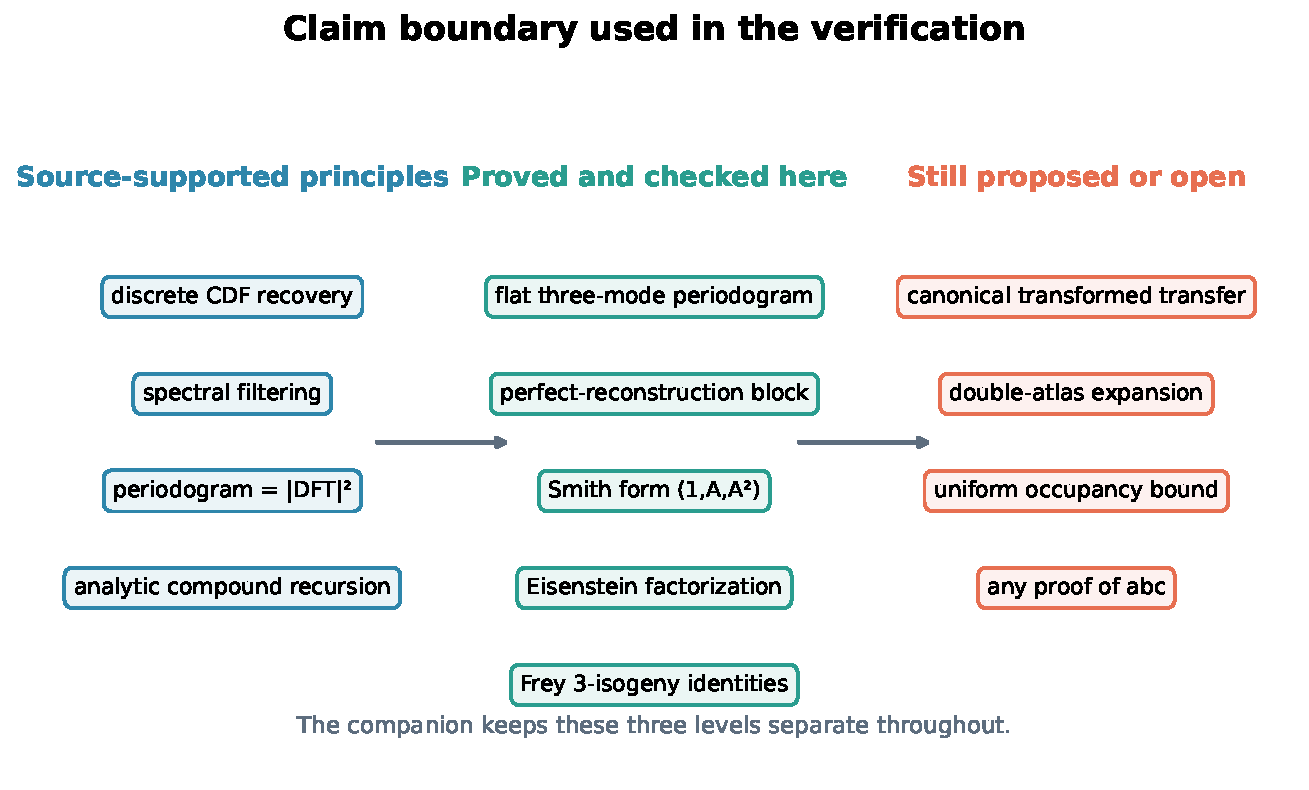
\includegraphics[width=0.96\textwidth]{figures/07_claim_status.pdf}
\caption{The three levels kept separate throughout the companion.}
\label{fig:claim-status}
\end{figure}

\section{Verification protocol}

The verification was carried out in four layers.

\subsection{Symbolic layer}

SymPy was used only as an exact polynomial algebra system.  The following identities were simplified to zero:

\begin{itemize}
  \item the general cyclic autocorrelation defect
  \item the general periodogram gap
  \item the perfect-reconstruction Gram identity after imposing $c=a+b$
  \item the Eisenstein DFT factorization
  \item the cubic harmonic identity
  \item the Frey invariant formulas
  \item the three Mordell-curve point equations
  \item the standard $3$-isogeny image
  \item the torsion translations
  \item the cubic fiber polynomial
  \item the torsion-orbit duplication product
\end{itemize}

No floating-point approximation is needed for any of these checks.

\subsection{Exact integer layer}

The full identity set was checked on $250$ randomly generated coprime pairs with $1\leq a,b\leq5000$.  For every pair, $c=a+b$ was formed and the following were recomputed independently:

\begin{itemize}
  \item the periodogram
  \item the circulant Gram matrix
  \item the Smith normal form
  \item all three Mordell points
  \item the support gcd statements
  \item the cubic identity $L^2+27a^2b^2c^2=4A^3$
\end{itemize}

All $250$ tests passed.

\subsection{Representation-count layer}

For every integer $1\leq A\leq400$, every pair $(a,b)$ in a box large enough to contain all solutions of
\[
  a^2+ab+b^2=A
\]
was enumerated.  The count was compared with the standard Eisenstein representation formula.  All $400$ values matched.

\subsection{Record-triple primality layer}

For the Reyssat triple, the transformed scale is
\[
  A=41{,}426{,}498{,}340{,}967.
\]
Its integer square root is
\[
  \lfloor\sqrt A\rfloor=6{,}436{,}342.
\]
A direct trial-division certificate checked all $440{,}708$ primes up to this bound.  The largest checked prime was $6{,}436{,}327$, and none divided $A$.  Thus the statement that this $A$ is prime was verified without relying on a probable-prime label.

\section{A bounded exact-zero projector before the three-channel reduction}

This section records one earlier claim because it explains why the later three-frequency construction is valuable.

Let $\Omega$ be a finite assignment set, and let the integer-valued defect operator be diagonal on $\ell^2(\Omega)$:
\[
  \mathsf D|\omega\rangle=D(\omega)|\omega\rangle,
  \qquad D(\omega)\in\Z.
\]
Let $N_0$ be the number of zero defects.

\begin{proposition}[Rational zero projector]
For every integer $m\geq1$, define
\[
  \mathsf K_m=(I+\mathsf D^2)^{-m}.
\]
Then
\[
  0\leq \Tr\mathsf K_m-N_0\leq |\Omega|2^{-m}.
\]
\end{proposition}

\begin{proof}
The eigenvalue of $\mathsf K_m$ at an integer defect $d$ is $(1+d^2)^{-m}$.  It equals one at $d=0$.  If $d\neq0$, then $1+d^2\geq2$, so the eigenvalue is at most $2^{-m}$.  Summing over the nonzero defects gives the bound.
\end{proof}

The same operator can be written using the Cayley transform
\[
  \mathsf U=(\mathsf D-iI)(\mathsf D+iI)^{-1}
\]
as
\[
  \mathsf K_m=
  \left(\frac{I-\mathsf U}{2}\right)^m
  \left(\frac{I-\mathsf U^*}{2}\right)^m.
\]
This is a genuine bounded functional-calculus certificate.

\subsection{Why a global cosine expansion still becomes expensive}

At an exact solution, perturb one log-coordinate by $\delta$.  Along the output coordinate, the defect takes the form
\[
  D(\delta)=c(1-e^\delta).
\]
At
\[
  \delta_c=\log\left(1-\frac1c\right),
\]
we have $D(\delta_c)=1$ and $|\delta_c|=c^{-1}+O(c^{-2})$.  Therefore the function $(1+D(\delta)^2)^{-m}$ falls from $1$ to $2^{-m}$ across a width of order $1/c$.

Bernstein's inequality for trigonometric polynomials then forces degree $\Omega(c)$ for a uniform approximation on the physical log-coordinate.  On an interval whose width is comparable to $\log c$, this becomes an $\Omega(c\log c)$ term count.

This is a limitation of the coordinate system, not a failure of filtering.  The next section avoids it entirely for an individual triple.

\section{The exact three-channel signal}\label{sec:three-channel}

Let $a,b,c$ be nonzero integers.  Define
\[
  \boxed{\mathbf s(a,b,c)=\begin{pmatrix}ac\\bc\\-ab\end{pmatrix}.}
\]
Let the cyclic shift be
\[
  \tau(x_0,x_1,x_2)=(x_2,x_0,x_1).
\]

\begin{theorem}[Autocorrelation defect]
The nonzero cyclic autocorrelations satisfy
\[
  \langle\mathbf s,\tau\mathbf s\rangle
  =\langle\mathbf s,\tau^2\mathbf s\rangle
  =abc(c-a-b).
\]
Consequently,
\[
  a+b=c
  \quad\Longleftrightarrow\quad
  \langle\mathbf s,\tau\mathbf s\rangle=0.
\]
\end{theorem}

\begin{proof}
A direct expansion gives
\begin{align*}
\langle\mathbf s,\tau\mathbf s\rangle
&=(ac)(-ab)+(bc)(ac)+(-ab)(bc)\\
&=-a^2bc+abc^2-ab^2c\\
&=abc(c-a-b).
\end{align*}
The second nonzero shift gives the same expression because a length-three real sequence has equal lag-one and lag-two cyclic autocorrelations.
\end{proof}

The relation is therefore not represented by a narrow spectral spike.  It is represented by exact orthogonality in three dimensions.

\subsection{Flat periodogram}

Let
\[
  \omega=e^{2\pi i/3}
\]
and use the unnormalized DFT
\[
  \widehat s_k=\sum_{j=0}^2s_j\omega^{jk}.
\]

\begin{theorem}[Periodogram gap]
For arbitrary $a,b,c$,
\[
  |\widehat s_0|^2-|\widehat s_1|^2
  =3abc(c-a-b),
\]
and $|\widehat s_1|=|\widehat s_2|$.  Hence
\[
  \boxed{a+b=c
  \quad\Longleftrightarrow\quad
  |\widehat s_0|=|\widehat s_1|=|\widehat s_2|.}
\]
\end{theorem}

\begin{proof}
Let $r_0=\sum_j|s_j|^2$ and let $r_1=r_2=abc(c-a-b)$ be the two nonzero cyclic autocorrelations.  The DFT of the cyclic autocorrelation gives
\[
  |\widehat s_0|^2=r_0+r_1+r_2=r_0+2r_1
\]
and
\[
  |\widehat s_1|^2=r_0+r_1\omega+r_2\omega^2=r_0-r_1.
\]
Subtracting gives $3r_1$.  Conjugate symmetry gives $|\widehat s_1|=|\widehat s_2|$.
\end{proof}

\begin{figure}[H]
\centering
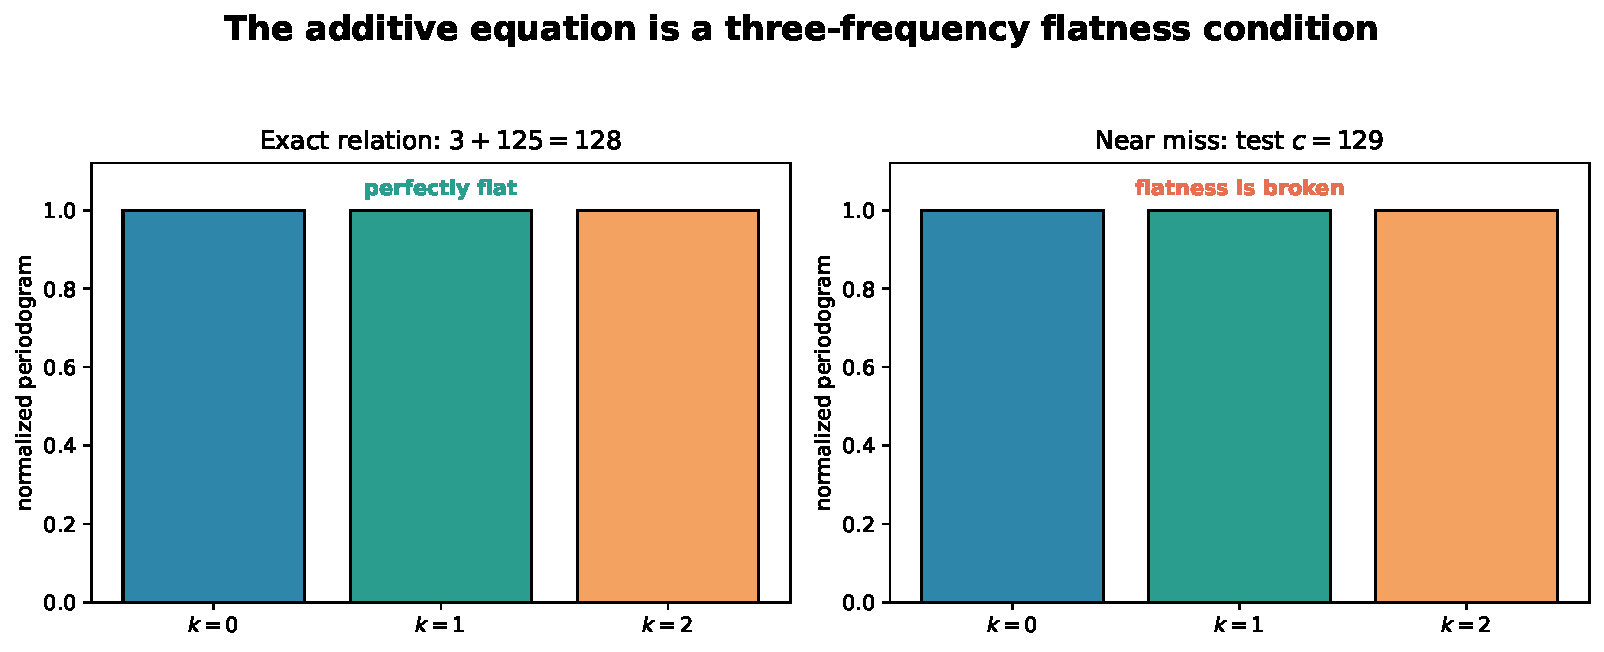
\includegraphics[width=0.94\textwidth]{figures/01_periodogram_flatness.pdf}
\caption{An exact triple gives a flat periodogram.  Perturbing only the output breaks flatness immediately.}
\label{fig:periodogram}
\end{figure}

\begin{remark}
The word ``periodogram'' is justified by the standard identity $P=|\DFT|^2$ in the supplied spectral notes \cite{Tibshirani2024}.  The number-theoretic equivalence above is a new calculation specific to this signal.
\end{remark}

\section{The circulant perfect-reconstruction block}

Assume from now on that $a,b$ are positive, $\gcd(a,b)=1$, and $c=a+b$.  Define
\[
  A=a^2+ab+b^2
\]
and
\[
  \boxed{
  \calC_{a,b,c}=
  \begin{pmatrix}
    ac&bc&-ab\\
    -ab&ac&bc\\
    bc&-ab&ac
  \end{pmatrix}.}
\]
The rows are the three cyclic shifts of $\mathbf s$.

\begin{theorem}[Perfect reconstruction]
For every primitive triple $a+b=c$,
\[
  \boxed{\calC\calC^T=A^2I_3.}
\]
Consequently,
\[
  \calC^{-1}=\frac{\calC^T}{A^2}
\]
and $\calC/A$ is an orthogonal matrix.
\end{theorem}

\begin{proof}
The off-diagonal Gram entries are the nonzero cyclic autocorrelations, so they vanish by the preceding theorem.  The diagonal entry is
\[
  a^2c^2+b^2c^2+a^2b^2.
\]
Using $c=a+b$ and expanding gives
\[
  a^2c^2+b^2c^2+a^2b^2=(a^2+ab+b^2)^2=A^2.
\]
\end{proof}

\begin{figure}[H]
\centering
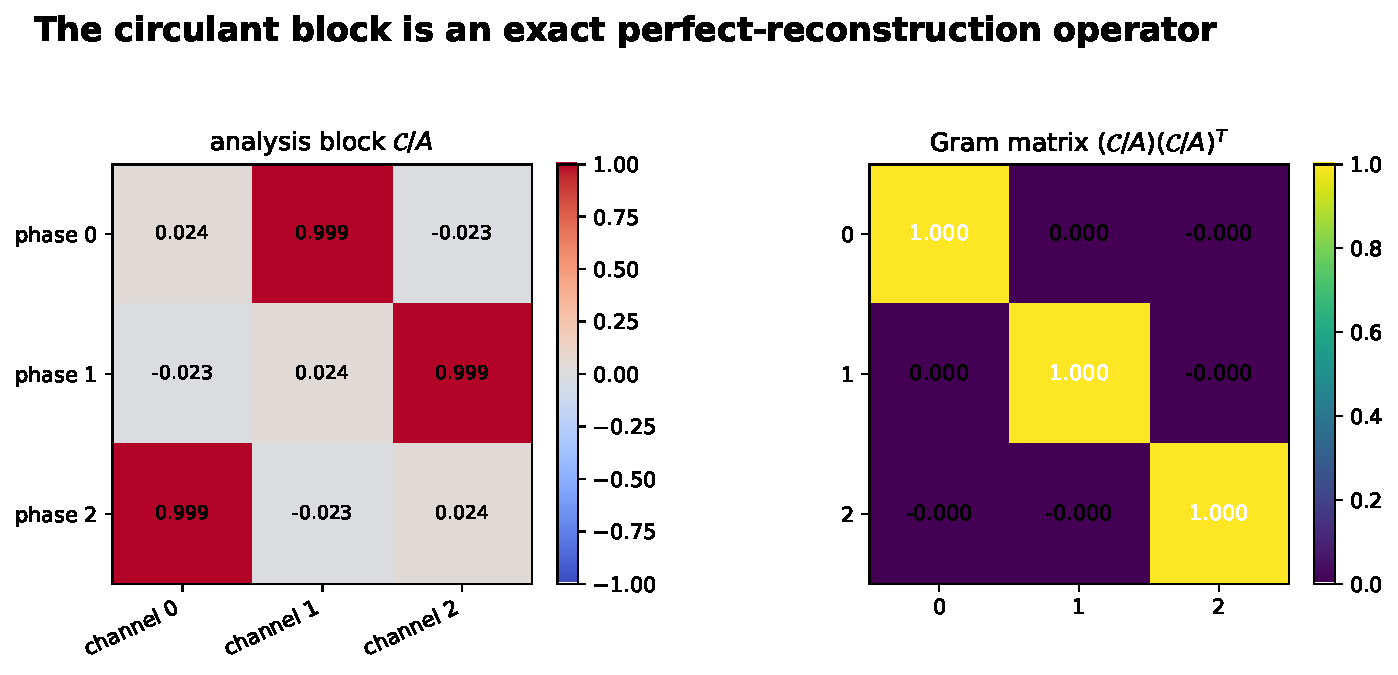
\includegraphics[width=0.94\textwidth]{figures/02_perfect_reconstruction.pdf}
\caption{The normalized analysis block and its exact identity Gram matrix for $3+125=128$.}
\label{fig:perfect-reconstruction}
\end{figure}

\subsection{Determinant and Smith form}

The DFT diagonalizes every circulant matrix.  We will soon identify the three eigenvalues as $A,z^2,\bar z^2$.  Their product is $A^3$, so
\[
  \det\calC=A^3.
\]
The same conclusion follows by taking determinants in $\calC\calC^T=A^2I$ and checking the sign on a positive example.

\begin{theorem}[Smith normal form]
For a primitive triple,
\[
  \boxed{\SNF(\calC)=\operatorname{diag}(1,A,A^2).}
\]
\end{theorem}

\begin{proof}
The gcd of the entries $ab,ac,bc$ is one because $a,b,c$ are pairwise coprime.  Hence the first Smith invariant is $d_1=1$.

From perfect reconstruction,
\[
  \operatorname{adj}(\calC)
  =\det(\calC)\calC^{-1}
  =A\calC^T.
\]
The entries of $\operatorname{adj}(\calC)$ are the signed $2\times2$ minors.  Their gcd is therefore $A$ times the gcd of the entries of $\calC$, namely $A$.  Hence
\[
  d_1d_2=A,
\]
so $d_2=A$.  Finally,
\[
  d_1d_2d_3=|\det\calC|=A^3,
\]
which gives $d_3=A^2$.
\end{proof}

The Smith form is exact, but its interpretation needs care.  It identifies one free integral channel and two weighted channels.  It does not by itself bound $A$ in terms of $\rad(abc)$.

\section{Eisenstein factorization of the Fourier modes}

Let
\[
  \zeta=e^{\pi i/3}=\frac{1+\sqrt{-3}}2
\]
and define
\[
  z=a+b\zeta.
\]
Then
\[
  z\bar z=a^2+ab+b^2=A.
\]

\begin{theorem}[Exact DFT factorization]
Under the ordering $\mathbf s=(ac,bc,-ab)$,
\[
  \boxed{(\widehat s_0,\widehat s_1,\widehat s_2)
  =(A,z^2,\bar z^{\,2}).}
\]
\end{theorem}

\begin{proof}
The constant channel is
\[
  \widehat s_0=ac+bc-ab=c^2-ab=A.
\]
Writing $\omega=e^{2\pi i/3}$ and using $\zeta=1+\omega$, a direct expansion gives
\[
  z^2=ac+bc\omega-ab\omega^2=\widehat s_1.
\]
Complex conjugation gives the third channel.
\end{proof}

The flat periodogram is now immediate:
\[
  |z^2|=|z|^2=A.
\]

\begin{figure}[H]
\centering
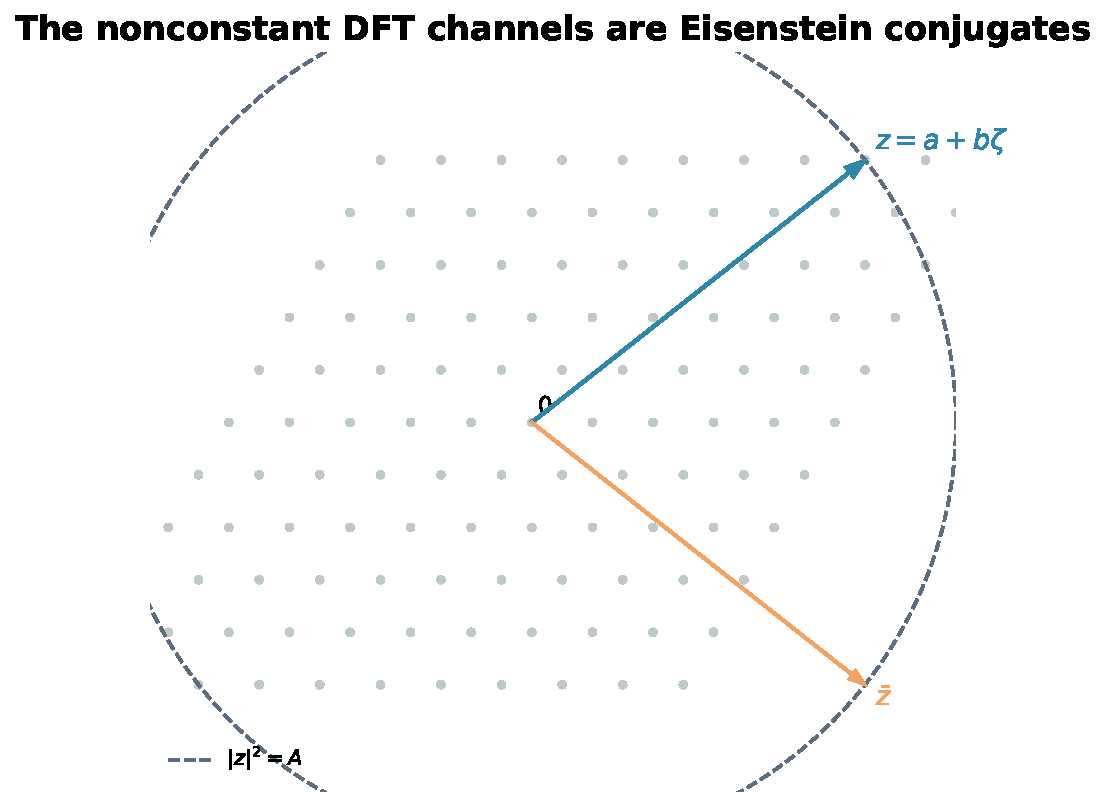
\includegraphics[width=0.75\textwidth]{figures/03_eisenstein_geometry.pdf}
\caption{The two nonconstant channels are conjugate points on the Eisenstein norm circle.}
\label{fig:eisenstein}
\end{figure}

\subsection{The third harmonic}

Define
\[
  L=(a-b)(a+2b)(2a+b).
\]

\begin{theorem}[Cubic harmonic identity]
\[
  \boxed{2z^3=L+3\sqrt{-3}\,abc.}
\]
Consequently,
\[
  \boxed{L^2+27a^2b^2c^2=4A^3.}
\]
\end{theorem}

\begin{proof}
Expand $z^3$ using $\zeta^2-\zeta+1=0$.  The real part simplifies to $L/2$, while the coefficient of $\sqrt{-3}$ is $3abc/2$.  Taking norms gives
\[
  4\Norm(z)^3=L^2+27a^2b^2c^2.
\]
Since $\Norm(z)=A$, the result follows.
\end{proof}

\begin{figure}[H]
\centering
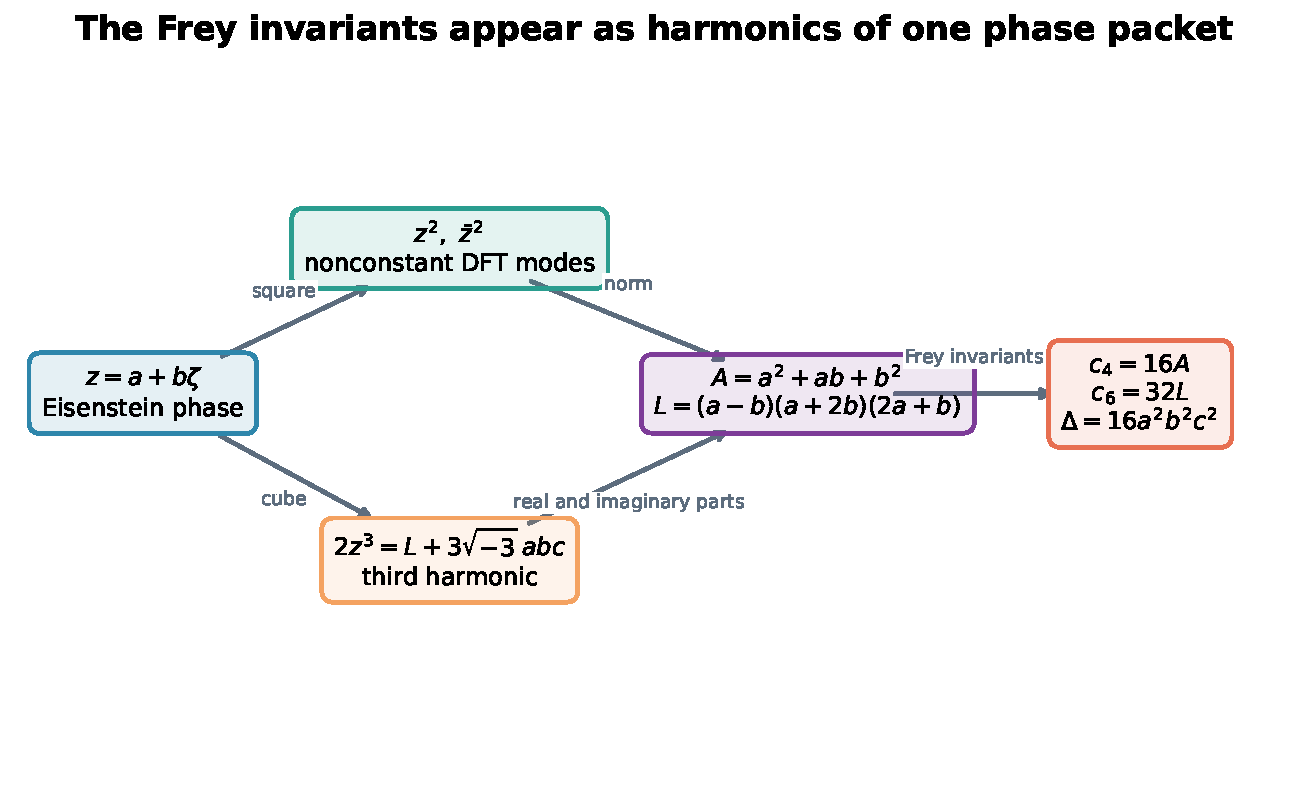
\includegraphics[width=0.97\textwidth]{figures/04_harmonic_to_frey.pdf}
\caption{The square and cube of one Eisenstein phase packet produce the DFT modes and the Frey invariants.}
\label{fig:harmonic-flow}
\end{figure}

\section{The Frey invariants are encoded in the third harmonic}

Consider the Frey curve
\[
  E_F:\qquad y^2=x(x-a)(x+b)
  =x^3+(b-a)x^2-abx.
\]

\begin{theorem}[Frey invariants]
The displayed integral model has
\[
  \boxed{c_4=16A,\qquad c_6=32L,\qquad
  \Delta_F=16a^2b^2c^2.}
\]
Moreover,
\[
  c_4^3-c_6^2=1728\Delta_F.
\]
\end{theorem}

\begin{proof}
For the Weierstrass coefficients
\[
  a_1=a_3=a_6=0,\qquad a_2=b-a,\qquad a_4=-ab,
\]
we have
\[
  b_2=4(b-a),\qquad b_4=-2ab,\qquad b_6=0,\qquad b_8=-a^2b^2.
\]
Substitution into the standard invariant formulas gives the displayed values.  The invariant relation is also the cubic harmonic identity multiplied by the appropriate powers of $2$.
\end{proof}

This is one of the strongest verified structural statements in the companion.  The Frey invariants are not being introduced from outside the signal construction.  They are already present in the third Eisenstein harmonic.

\section{The Mordell curve and the rational \texorpdfstring{$3$}{3}-isogeny}

Set
\[
  \kappa=4abc
\]
and consider
\[
  \calM_\kappa:\qquad V^2=U^3+\kappa^2.
\]
Define
\[
\begin{aligned}
P_{bc}&=(4bc,\,4bc(a+2b)),\\
P_{ac}&=(4ac,\,4ac(2a+b)),\\
P_{ab}&=(-4ab,\,4ab(a-b)).
\end{aligned}
\]

\begin{proposition}[Three integral sector points]
All three points lie on $\calM_\kappa$.
\end{proposition}

\begin{proof}
For example,
\[
  [4bc(a+2b)]^2-(4bc)^3-(4abc)^2=0
\]
after factoring out $16b^2c^2$ and using $c=a+b$.  The other two identities are the corresponding permutations.  The verification script checks all three symbolically.
\end{proof}

\subsection{The standard \texorpdfstring{$3$}{3}-isogeny}

The point
\[
  T=(0,\kappa)
\]
has order three on $\calM_\kappa$.  The standard isogeny with kernel $\langle T\rangle$ is
\[
  \phi(U,V)=
  \left(
    \frac{U^3+4\kappa^2}{U^2},
    \frac{V(U^3-8\kappa^2)}{U^3}
  \right),
\]
with target
\[
  \calM_\kappa':\qquad Y^2=X^3-27\kappa^2.
\]

\begin{theorem}[Invariant-point image]
\[
  \boxed{\phi(P_{bc})=(4A,-4L)
  =\left(\frac{c_4}{4},-\frac{c_6}{8}\right).}
\]
The same image is obtained from the other two sector points after the torsion translations described below.
\end{theorem}

\begin{proof}
Substitute $U=4bc$, $V=4bc(a+2b)$, and $\kappa=4abc$ into the isogeny formulas.  Cancelling the common powers of $4bc$ gives
\[
  X=4(a^2+ab+b^2)=4A
\]
and
\[
  Y=-4(a-b)(a+2b)(2a+b)=-4L.
\]
\end{proof}

\subsection{The torsion orbit}

\begin{theorem}[Sector orbit]
\[
  \boxed{P_{bc}+T=-P_{ab},\qquad
  P_{bc}+2T=-P_{ac}.}
\]
\end{theorem}

\begin{proof}
Use the ordinary chord-and-tangent addition law on $V^2=U^3+\kappa^2$.  For $P_{bc}+T$, the slope is
\[
  m=\frac{4bc(a+2b)-\kappa}{4bc}=2b.
\]
The resulting $U$-coordinate is
\[
  m^2-4bc=4b^2-4bc=-4ab,
\]
and the resulting $V$-coordinate is $-4ab(a-b)$, which is the negative of the $V$-coordinate of $P_{ab}$.  The second identity is analogous, or follows by adding $T$ once more.
\end{proof}

\begin{figure}[H]
\centering
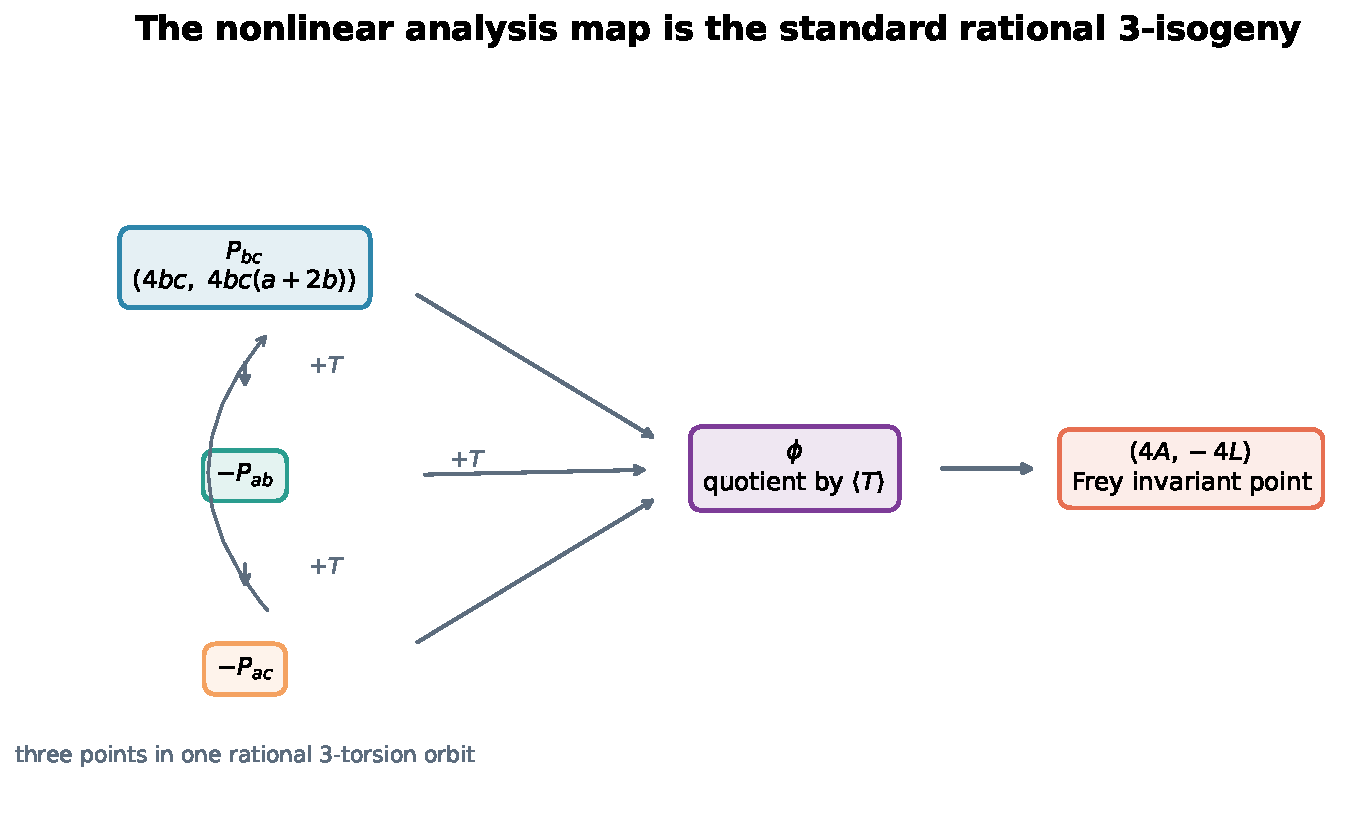
\includegraphics[width=0.97\textwidth]{figures/05_isogeny_fiber.pdf}
\caption{The three sector points differ by rational $3$-torsion and have the same isogeny image.}
\label{fig:isogeny}
\end{figure}

\subsection{Perfect reconstruction from the fiber}

The three $U$-coordinates are
\[
  4bc,\qquad4ac,\qquad-4ab.
\]

\begin{theorem}[Fiber cubic]
They are the roots of
\[
  \boxed{t^3-4At^2+4\kappa^2=0.}
\]
\end{theorem}

\begin{proof}
Their sum is
\[
  4bc+4ac-4ab=4A.
\]
Their pairwise-product sum vanishes:
\[
  16abc(c-a-b)=0.
\]
Their product is
\[
  -64a^2b^2c^2=-4\kappa^2.
\]
Vieta's formulas give the polynomial.
\end{proof}

The zero coefficient of $t$ is the additive equation in symmetric form.  Analysis maps three sector products to one invariant point.  Synthesis recovers the sector products as the roots of the fiber cubic, with the expected torsion ambiguity.

\subsection{A norm over the torsion orbit}

Let $\psi_2(U,V)=2V$ be the duplication division polynomial.

\begin{theorem}[Torsion-orbit product]
\[
  \boxed{\prod_{j=0}^2\psi_2(P_{bc}+jT)=\Delta_Fc_6.}
\]
\end{theorem}

\begin{proof}
Using the orbit points,
\begin{align*}
\prod_{j=0}^2\psi_2(P_{bc}+jT)
&=[8bc(a+2b)][-8ab(a-b)][-8ac(2a+b)]\\
&=512a^2b^2c^2L\\
&=(16a^2b^2c^2)(32L)\\
&=\Delta_Fc_6.
\end{align*}
\end{proof}

\section{Prime-support separation in the transformed atlas}

The original radical and the transformed quantities $A$ and $L$ have unusually clean gcd relations.

\begin{theorem}[Support separation]
For every primitive positive triple $a+b=c$,
\[
  \boxed{\gcd(A,abc)=1,}
\]
\[
  \boxed{\gcd(L,abc)=2,}
\]
and
\[
  \boxed{\gcd(A,L)\in\{1,3\}.}
\]
\end{theorem}

\begin{proof}
If $p\mid a$, then $A\equiv b^2\pmod p$, which is nonzero.  The same argument works for $p\mid b$.  If $p\mid c$, then $a\equiv-b\pmod p$, so $A\equiv a^2\pmod p$.  This proves $\gcd(A,abc)=1$.

No odd prime dividing $a$, $b$, or $c$ can divide any of the three factors of $L$.  For instance, if $p\mid a$, then the factors of $L$ reduce to $-b$, $2b$, and $b$ modulo $p$.  The other sectors are similar.  A parity check shows that $L$ and $abc$ share exactly one factor of $2$.  Hence $\gcd(L,abc)=2$.

If a prime divides both $A$ and $L$, the identity
\[
  4A^3-L^2=27a^2b^2c^2
\]
and $\gcd(A,abc)=1$ show that the prime must be $3$.  Finally, $v_3(A)\leq1$ for coprime $a,b$.  Therefore the common gcd is $1$ or $3$.
\end{proof}

\begin{figure}[H]
\centering
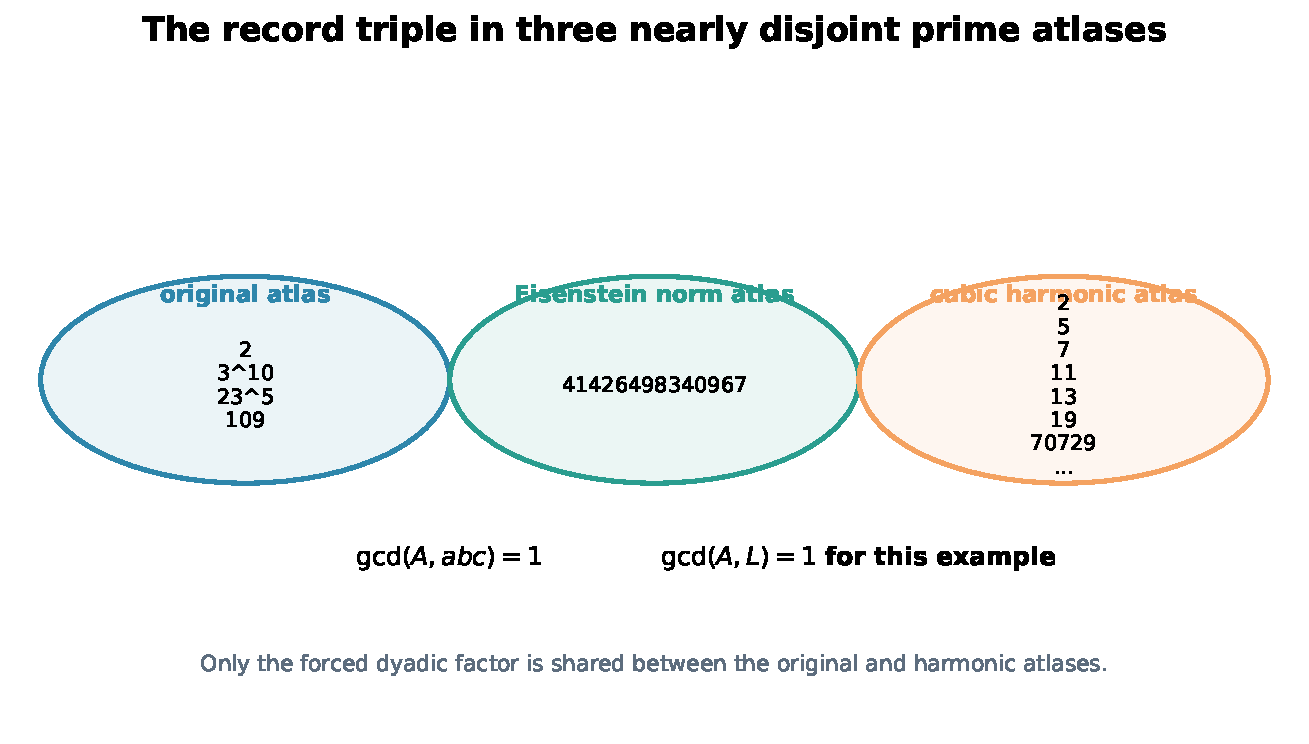
\includegraphics[width=0.97\textwidth]{figures/06_support_atlases.pdf}
\caption{The record triple produces three nearly disjoint prime atlases.}
\label{fig:support-atlases}
\end{figure}

\section{Uniform lifting in the Eisenstein atlas}

Let $q$ be a prime divisor of $A$.

\begin{theorem}[Prime classification]
If $q\neq3$, then
\[
  \boxed{q\equiv1\pmod3.}
\]
Moreover, the ratio $t\equiv ab^{-1}\pmod q$ is a simple root of
\[
  f(T)=T^2+T+1.
\]
It therefore lifts uniquely to every modulus $q^n$.
\end{theorem}

\begin{proof}
Since $\gcd(A,b)=1$, the ratio $t=ab^{-1}$ is defined modulo $q$.  The congruence $q\mid A$ becomes
\[
  t^2+t+1\equiv0\pmod q.
\]
Thus $t^3\equiv1\pmod q$.  If $q\neq3$, then $t\not\equiv1$, so the multiplicative group modulo $q$ contains an element of order three.  Therefore $3\mid q-1$.

The derivative is $f'(t)=2t+1$.  If $f(t)\equiv f'(t)\equiv0\pmod q$, substitution gives $3\equiv0\pmod q$.  This is excluded.  Hensel's lemma gives a unique lift through all powers of $q$.
\end{proof}

\begin{corollary}[Factorization shape]
For a primitive triple,
\[
  \boxed{A=3^\delta\prod_{q\equiv1\pmod3}q^{f_q},
  \qquad \delta\in\{0,1\}.}
\]
\end{corollary}

\begin{proof}
The prime classification handles every $q\neq3$.  To see $v_3(A)\leq1$, note that $3\mid A$ implies $a\equiv b\pmod3$ and neither is divisible by $3$.  Write $a=b+3k$.  Then
\[
  A=3(b^2+3bk+3k^2),
\]
and the factor in parentheses is nonzero modulo $3$.
\end{proof}

\section{Representation count in the transformed atlas}

The ring of Eisenstein integers is a unique factorization domain with six units.  The norm of $a+b\zeta$ is $a^2+ab+b^2$.

\begin{theorem}[Representation count]
Suppose
\[
  A=3^\delta\prod_{j=1}^r q_j^{f_j},
  \qquad q_j\equiv1\pmod3,
  \qquad \delta\in\{0,1\}.
\]
Then the number of ordered integer pairs $(a,b)$ satisfying
\[
  a^2+ab+b^2=A
\]
is
\[
  \boxed{6\prod_{j=1}^r(f_j+1).}
\]
In particular, for every $\eta>0$,
\[
  \#\{(a,b):a^2+ab+b^2=A\}\ll_\eta A^\eta.
\]
\end{theorem}

\begin{proof}
Every split prime $q_j$ factors as $\pi_j\bar\pi_j$.  In an element of norm $A$, the exponent $f_j$ may be divided between $\pi_j$ and $\bar\pi_j$ in exactly $f_j+1$ ways.  The ramified factor above $3$ contributes no additional binary choice.  Multiplication by one of the six units gives the factor $6$.  Unique factorization shows that these are all representations.
\end{proof}

The exact formula was checked by brute force for every $1\leq A\leq400$.

\section{Worked examples}

\begin{table}[H]
\centering
\small
\begin{tabular}{rrrrrrr}
\toprule
$a$ & $b$ & $c$ & $A$ & $\rad(abc)$ & $q$ & $\gcd(A,L)$\\
\midrule
1 & 1 & 2 & 3 & 2 & 1.000000 & 3\\
1 & 8 & 9 & 73 & 6 & 1.226294 & 1\\
2 & 3 & 5 & 19 & 30 & 0.473197 & 1\\
3 & 125 & 128 & 16009 & 30 & 1.426565 & 1\\
121 & 48234375 & 48234496 & 2326560768014641 & 53130 & 1.625991 & 1\\
2 & 6436341 & 6436343 & 41426498340967 & 15042 & 1.629912 & 1\\
\bottomrule
\end{tabular}
\caption{Worked examples used in the exact audit.  Here $q=\log c/\log\rad(abc)$.}
\label{tab:worked}
\end{table}

\begin{figure}[H]
\centering
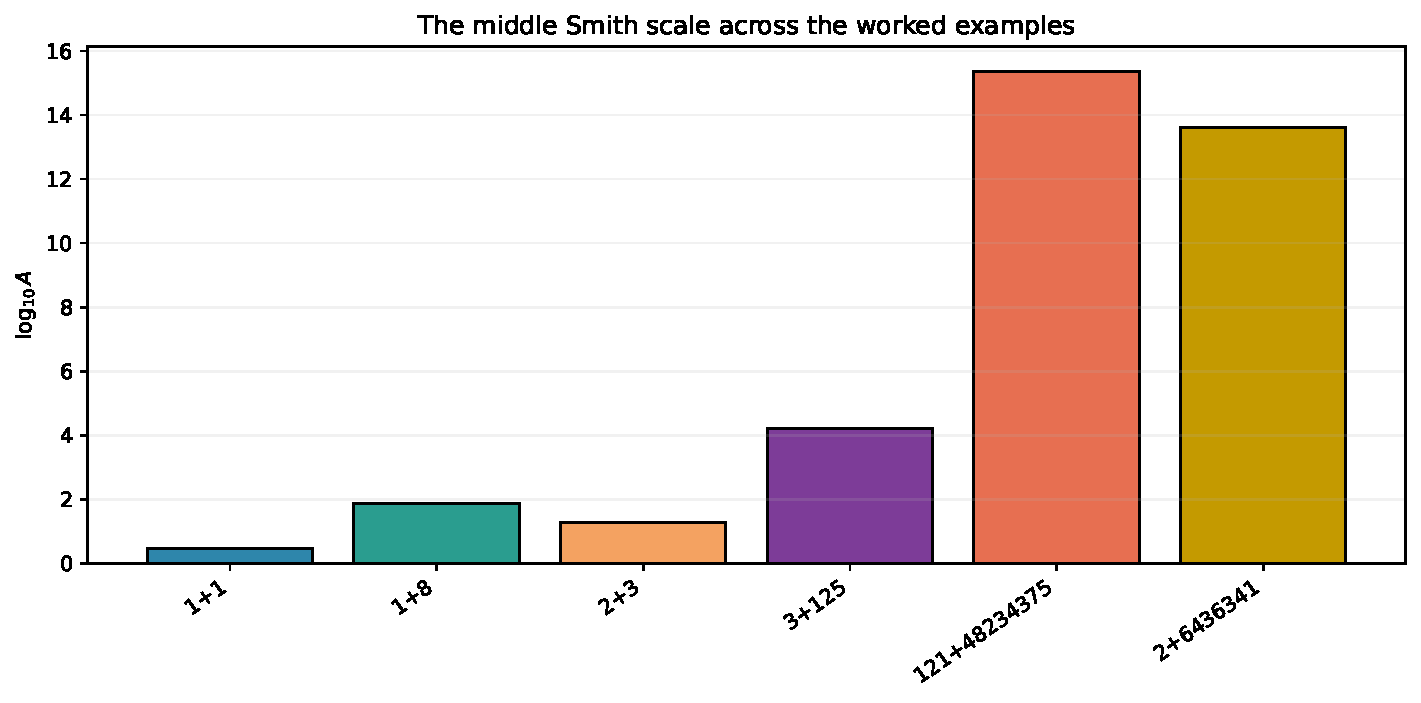
\includegraphics[width=0.88\textwidth]{figures/08_worked_smith_scales.pdf}
\caption{The middle Smith scale $A$ across the worked examples.}
\label{fig:worked-scales}
\end{figure}

\subsection{The Reyssat triple}

For
\[
  2+3^{10}\cdot109=23^5,
\]
we have
\[
  a=2,
  \qquad b=6{,}436{,}341,
  \qquad c=6{,}436{,}343.
\]
The original radical is
\[
  \rad(abc)=2\cdot3\cdot23\cdot109=15{,}042.
\]
The middle Smith scale is
\[
  \boxed{A=41{,}426{,}498{,}340{,}967.}
\]
It is prime and congruent to one modulo three.

The cubic harmonic is
\[
  L=-533{,}270{,}222{,}369{,}637{,}973{,}220
\]
with factorization
\[
  |L|=2^2\cdot5\cdot7\cdot11\cdot13\cdot19
  \cdot67{,}751\cdot70{,}729\cdot292{,}561.
\]
The original and transformed prime supports are therefore almost completely disjoint.

This is a strong structural compression.  It does not imply that the triple is impossible.  In fact, it shows why the triple is rigid in the transformed atlas: the norm $A$ has only one split prime factor.

\section{What the verified identities do and do not establish}

\subsection{What is now proved}

The following statements are established without conjectural input:

\begin{enumerate}
  \item $a+b=c$ is equivalent to zero nontrivial cyclic autocorrelation of $\mathbf s$.
  \item $a+b=c$ is equivalent to a flat three-point periodogram.
  \item The circulant block has exact perfect reconstruction.
  \item Its Smith normal form is $\operatorname{diag}(1,A,A^2)$ for primitive triples.
  \item The DFT factors as $(A,z^2,\bar z^2)$.
  \item The third harmonic gives $L$ and $abc$ through $2z^3=L+3\sqrt{-3}abc$.
  \item The Frey invariants are $16A$, $32L$, and $16a^2b^2c^2$.
  \item The three Mordell points form one rational $3$-torsion orbit.
  \item The standard $3$-isogeny maps that orbit to $(4A,-4L)$.
  \item The fiber cubic reconstructs the three sector products.
  \item The torsion-orbit duplication product equals $\Delta_Fc_6$.
  \item The support gcd and Eisenstein lifting statements hold.
  \item The representation count is subpolynomial in $A$.
\end{enumerate}

\subsection{What remains a proposal}

The phrase ``double-atlas expansion'' describes a plausible future program, not a proved theorem.  To turn it into mathematics one must first specify:

\begin{itemize}
  \item the finite state space on which the transformed transfer acts
  \item the probability or counting measure being averaged
  \item the exact local multiplier at every prime in the $A$-atlas
  \item the rigid subspace that must be removed
  \item the norm in which contraction is measured
  \item the global occupancy inequality that converts contraction into an $abc$ bound
\end{itemize}

Without those definitions, the number $1/(q-1)$ is only a familiar Ramanujan-sum scale.  It is not yet a canonical invariant of one triple.

\subsection{Why this is not a proof of \texorpdfstring{$abc$}{abc}}

The middle Smith scale satisfies
\[
  A=c^2-ab,
\]
so
\[
  \frac34c^2\leq A<c^2.
\]
A bound
\[
  A\ll_\varepsilon\rad(abc)^{2+\varepsilon}
\]
would imply strong $abc$, after a harmless change of $\varepsilon$.  Conversely, strong $abc$ gives a bound of this shape.  The present identities reveal $A$ in several coordinate systems.  They do not yet bound it by the original radical.

That is the remaining arithmetic step.

\section{A refined research target}

The verified construction suggests a cleaner target than the earlier informal statement.

Let
\[
  S_0=\operatorname{supp}(abc),
  \qquad
  S_1=\operatorname{supp}(A).
\]
The two supports are disjoint.  At the original primes, the earlier lift calculus produces additive residue packets.  At the transformed primes, the Eisenstein equation produces two lifted cubic phases.  A future theorem would have to show one of two things:

\begin{enumerate}
  \item sufficiently many primes are transverse in at least one atlas, causing a quantitatively strong contraction
  \item the packet is rigid in both atlases, forcing it into a bounded-complexity bi-$S$-unit family that can be closed by arithmetic-curve methods
\end{enumerate}

This is a well-motivated program.  It is not yet a theorem.  The companion leaves it in that form rather than turning it into a conclusion.

\section{Reproducibility ledger}

The release contains:

\begin{itemize}
  \item the complete LaTeX source
  \item the exact symbolic and integer verification script
  \item the figure-generation script
  \item CSV tables for the worked examples, random audit, and representation formula
  \item the machine-readable JSON result ledger
  \item vector and PNG copies of every figure
\end{itemize}

The exact run completed with:

\begin{center}
\begin{tabular}{lr}
\toprule
Check group & Count\\
\midrule
Symbolic theorem chain & 1 complete chain\\
Random primitive triples & 250\\
Worked triples & 6\\
Representation-count values & 400\\
Trial-division primes for record $A$ & 440{,}708\\
Figure pairs & 8\\
\bottomrule
\end{tabular}
\end{center}

All checks passed.

\appendix

\section{Compact derivation sheet}

For convenient reference, the main identities are collected here.

\subsection*{Signal layer}
\[
\mathbf s=(ac,bc,-ab)^T,
\qquad
\langle\mathbf s,\tau\mathbf s\rangle=abc(c-a-b).
\]
\[
|\widehat s_0|^2-|\widehat s_1|^2=3abc(c-a-b).
\]

\subsection*{Perfect-reconstruction layer}
\[
A=a^2+ab+b^2,
\qquad
\calC\calC^T=A^2I_3,
\qquad
\SNF(\calC)=\operatorname{diag}(1,A,A^2).
\]

\subsection*{Eisenstein layer}
\[
\zeta=\frac{1+\sqrt{-3}}2,
\qquad
z=a+b\zeta,
\qquad
z\bar z=A.
\]
\[
(\widehat s_0,\widehat s_1,\widehat s_2)=(A,z^2,\bar z^2).
\]
\[
2z^3=L+3\sqrt{-3}\,abc,
\qquad
L=(a-b)(a+2b)(2a+b).
\]
\[
L^2+27a^2b^2c^2=4A^3.
\]

\subsection*{Frey and isogeny layer}
\[
c_4=16A,
\qquad
c_6=32L,
\qquad
\Delta_F=16a^2b^2c^2.
\]
\[
\kappa=4abc,
\qquad
\calM_\kappa:V^2=U^3+\kappa^2.
\]
\[
\phi(U,V)=
\left(
\frac{U^3+4\kappa^2}{U^2},
\frac{V(U^3-8\kappa^2)}{U^3}
\right).
\]
\[
\phi(P_{bc})=(4A,-4L).
\]
\[
(t-4bc)(t-4ac)(t+4ab)=t^3-4At^2+4\kappa^2.
\]
\[
\prod_{j=0}^2\psi_2(P_{bc}+jT)=\Delta_Fc_6.
\]

\section{Claim ledger}

\begin{longtable}{>{\raggedright\arraybackslash}p{0.28\textwidth}>{\raggedright\arraybackslash}p{0.19\textwidth}>{\raggedright\arraybackslash}p{0.42\textwidth}}
\toprule
Statement & Status & Basis\\
\midrule
\endfirsthead
\toprule
Statement & Status & Basis\\
\midrule
\endhead
Discrete CDF recovery is preferable to direct PMF filtering at atoms & Source-supported & Shen--Fang--Liu prove the discrete-CDF convergence framework and explain the atom problem.\\
Periodogram equals squared DFT modulus & Source-supported & Standard spectral identity stated in the supplied lecture notes.\\
Analytic coefficients can be propagated through compound COS stages & Source-supported & Huang--Oosterlee derive the quadrature-free recursion.\\
Digital payoff coefficients can be analytic & Source-supported & Fang's thesis gives the coefficients explicitly.\\
Autocorrelation defect identity & Proved & Direct expansion.\\
Flat-periodogram equivalence & Proved & DFT of the cyclic autocorrelation.\\
Perfect-reconstruction Gram identity & Proved & Orthogonality plus diagonal norm calculation.\\
Smith form $(1,A,A^2)$ & Proved & Entry gcd, adjugate, determinant.\\
DFT factorization $(A,z^2,\bar z^2)$ & Proved & Eisenstein expansion.\\
Cubic harmonic and Frey invariants & Proved & Exact polynomial expansion.\\
Mordell points and $3$-isogeny image & Proved & Exact substitution.\\
Torsion orbit and fiber cubic & Proved & Group law and Vieta.\\
Support separation and prime classification & Proved & Elementary congruences and Hensel's lemma.\\
Record $A$ is prime & Computed exactly & Trial division through $\lfloor\sqrt A\rfloor$.\\
Transformed multiplier $1/(q-1)$ is canonical & Not proved & Requires a specified transfer measure.\\
Double-atlas expansion--rigidity theorem & Open proposal & No uniform contraction or occupancy theorem has been established.\\
The $abc$ conjecture follows from the present companion & False & The required bound on the Smith scale $A$ remains open.\\
\bottomrule
\end{longtable}

\section{Complete verification code}

The following script generated the symbolic ledger, random checks, worked-example table, representation-count checks, and record-triple primality certificate.

\lstinputlisting[style=companion]{verify_three_channel_companion.py}

\section{Source map}

The source papers are cited for the following limited purposes.

\begin{itemize}
  \item Shen--Fang--Liu: discrete CDF recovery, spectral filters, PMF-at-atom caution, multivariate extension
  \item Tibshirani: finite Fourier decomposition and periodogram identity
  \item Huang--Oosterlee: analytic multi-stage coefficient propagation and stability
  \item Fang: characteristic-function sampling of cosine coefficients, digital payoff coefficients, and classical COS error decomposition
\end{itemize}

None of the four sources states the arithmetic signal theorem, the Smith form, the Eisenstein factorization, the Mordell points, or the $3$-isogeny identities.  Those are proved and checked in this companion.

\begin{thebibliography}{9}

\bibitem{ShenFangLiu2024}
X. Shen, F. Fang, and C. Liu,
\emph{The Fourier Cosine Method for Discrete Probability Distributions},
arXiv:2410.04487v2, 2024.

\bibitem{Tibshirani2024}
R. Tibshirani,
\emph{Lecture 5: Spectral Analysis and Decomposition},
Introduction to Time Series, Fall 2024.

\bibitem{HuangOosterlee2026}
Z. Huang and C. W. Oosterlee,
\emph{An Analytic COS Method for Compound Option Valuation},
arXiv:2607.25599v1, 2026.

\bibitem{Fang2010}
F. Fang,
\emph{The COS Method: An Efficient Fourier Method for Pricing Financial Derivatives},
Ph.D. thesis, Delft University of Technology, 2010.

\end{thebibliography}

\end{document}
